%%% Ne pas modifier jusqu'à la ligne 25
\documentclass[a4paper,12pt]{book}
\usepackage[utf8]{inputenc}
\usepackage[french]{babel}
%%\usepackage{CJK}
\usepackage{yhmath}
\usepackage[left=2cm,right=2cm,top=3cm,bottom=2cm, headheight=1.5cm,headsep=1.5cm]{geometry}
%%\usepackage{CJKutf8}
\usepackage{amsfonts}
\usepackage{esint}
\usepackage{mathrsfs}
\usepackage{amsmath,amsfonts,amssymb,dsfont}
\usepackage{graphicx}
\usepackage{subfigure}
\usepackage{enumitem}		%\enumerate-resume
\usepackage[colorlinks=true,unicode={true},hyperindex=false, linkcolor=blue, urlcolor=blue]{hyperref}
\newcommand{\myref}[1]{\ref{#1} page \pageref{#1}}

\addto\captionsfrench{\def\tablename{Tableau}}  %légendes des tableaux
\renewcommand\thesection{\Roman{section}~-~} 
\renewcommand\thesubsection{\Roman{section}.\Alph{subsection}~-~} 
\renewcommand\thesubsubsection{\Roman{section}.\Alph{subsection}.\arabic{subsubsection}~-~} 

\newcommand{\conclusion}[1]{\newline \centerline{\fbox{#1}}}

\setcounter{secnumdepth}{3}
\parindent=0pt

\usepackage{fancyhdr}
\pagestyle{fancy}

\lhead{SJTU-ParisTech} 
%%%%%%%%%%%%%%%%%%%%%%%%%%%%%%%%%%
\chead{DM4}
\rhead{Daniel 518261910024}

\begin{document}
\renewcommand{\labelitemi}{$\blacktriangleright$}
\renewcommand{\labelitemii}{$\bullet$}


\section{TD 1-10}
\begin{figure}[h]
    \begin{center}
    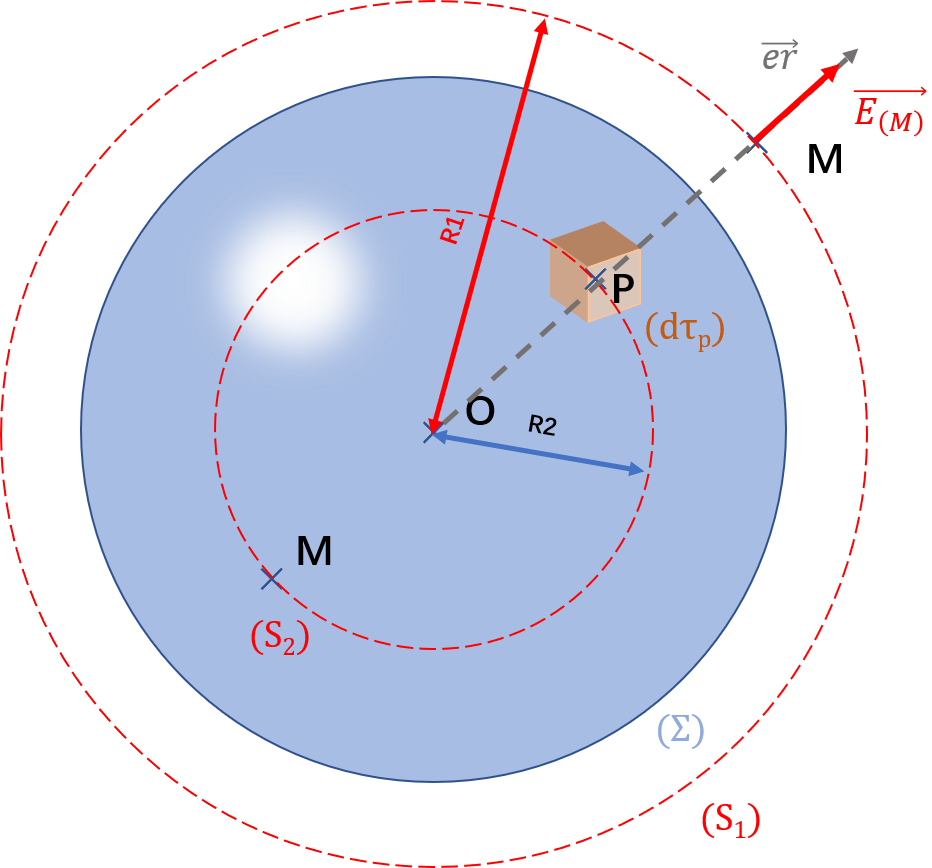
\includegraphics[scale=0.6]{elec21.png}
    \end{center}
    \caption{le système étudiée}
\end{figure}
\subsection{}
Le système $(\Sigma)$ étudiée: Le boule chargée

On a la charge élémentaire $\delta Q=\rho(P,t)\,d\tau_P$, avec $\rho(P,t)$ la densité volumique de charge.
Pour une répartie uniformément et supposant que la charge est indépendant du temps, on a $\rho(P,t)=\rho$

Dans le modèle d'une distribution de charge continue, on a 
$$
Q_{tot}=e=\iiint_{P \in (\Sigma)} \rho\,d\tau_P=\rho\iiint_{P \in (\Sigma)}d\tau_P=\frac{4}{3}\pi R^3\rho
$$
Donc la charge totale $\boxed{Q_{tot}=\frac{4}{3}\pi R^3\rho}$
\subsection{}
Pour un point $M=(r,\theta,\varphi)$ quelconque, le système $(\Sigma)$ est symmétrique par rapport à $O$, donc $\overrightarrow{E(M)}$ est selon la direction $\vec{e}_r$: $\overrightarrow{E(M)}=E(r,\theta,\varphi)\vec{e}_r$

Le système $(\Sigma)$ est invariante par rotation autour du point $O$, donc la norme du champ électrostatique $E(M)$ ne dépend que de la distance: $\overrightarrow{E(M)}=E(r)\vec{e}_r$ 

On va employer les coordonnées sphériques, et on a donc $\overrightarrow{E(M)}=E(R)\vec{e}_r$ par la symétrie
\begin{itemize}
    \item Cas 1: Soit $M=(R_1,\theta,\varphi)$ se trouve à l'extérieur de la boule, on pose $(S_1)$ la surface fermée qui passe par $M$, avec le rayon $R_1\geq R$. 
    $(S_1)$ est une surface iso-E comme tous les points sur $(S_1)$ ont la même distance par rapport à $O$. 
    Donc on a le flux qui traverse $(S_1)$
    $$
    \Phi_1=\varoiint_{M \in (S_1)} \overrightarrow{E(M)}\cdot \overrightarrow{dS_M}=\varoiint_{M \in (S_1)} E(R_1)\vec{e}_r\cdot dS\vec{e}_r=4\pi R_1^2E(R_1)
    $$
    et selon le théorème de Gauss, on a aussi
    $$
    \Phi_1=\frac{Q_{int}}{\epsilon_0}=\frac{Q_{tot}}{\epsilon_0}=\frac{4\pi R^3\rho}{3\epsilon_0}
    $$
    On a donc 
    $$
    4\pi R_1^2E(R_1)=\frac{4\pi R^3\rho}{3\epsilon_0}
    $$
    d'où
    $$
    \boxed{E(R_1)=\frac{R^3\rho}{3R_1^2\epsilon_0}}
    $$
    \item Cas 2: Soit $M=(R_2,\theta,\varphi)$ se trouve à l'intérieur de la boule, on pose $(S_2)$ la surface fermée qui passe par $M$, avec le rayon $R_2 < R$. 
    $(S_2)$ est une surface iso-E comme tous les points sur $(S_2)$ ont la même distance par rapport à $O$. 
    Donc on a le flux qui traverse $(S_1)$
    $$
    \Phi_2=\varoiint_{M \in (S_2)} \overrightarrow{E(M)}\cdot \overrightarrow{dS_M}=\varoiint_{M \in (S_2)} E(R_2)\vec{e}_r\cdot dS\vec{e}_r=4\pi R_2^2E(R_2)
    $$
    et selon le théorème de Gauss, on a aussi
    $$
    \Phi_1=\frac{Q_{int}}{\epsilon_0}=\frac{4\pi R_2^3\rho}{3\epsilon_0}
    $$
    On a donc 
    $$
    4\pi R_2^2E(R_2)=\frac{4\pi R_2^3\rho}{3\epsilon_0}
    $$
    d'où
    $$
    \boxed{E(R_2)=\frac{R_2\rho}{3\epsilon_0}}
    $$
\end{itemize}
On a donc pour $M=(r,\theta,\varphi)$ quelconque
\begin{equation}  \nonumber
    \boxed{\overrightarrow{E(M)}=\left\{  
                 \begin{array}{rcl}  
                    \frac{R^3\rho}{3r^2\epsilon_0}\vec{e}_r & & r \geq R\\
                    \frac{r\rho}{3\epsilon_0}\vec{e}_r & & 0\leq r<R\\
                 \end{array}  
    \right.  }
\end{equation}
On notice que $\overrightarrow{E(M)}$ est continue en $r=R$

\subsection{}
On a 
$$\overrightarrow{E(M)}=-\overrightarrow{grad}V(M)=-\left(\frac{\partial V}{\partial r}\vec{e}_r+\frac{1}{r}\frac{\partial V}{\partial \theta}\vec{e}_\theta+\frac{1}{r\sin\theta}\frac{\partial V}{\partial \varphi}\vec{e}_\varphi\right)$$
En faisant des projections, on a 
$$
\frac{\partial V}{\partial \theta}=0 \qquad \frac{\partial V}{\partial \varphi}=0
$$
Donc $V=V(r)$, $\frac{\partial V}{\partial r}=\frac{dV}{dr}$

Pour $r \geq R$, on a 
$$
\frac{R^3 \rho}{3r^2 \epsilon_0}=-\frac{dV}{dr}
$$
On a donc 
$$
\int_{V_\infty}^{V(r)}dV=-\int_{r_\infty}^{r}\frac{R^3 \rho}{3r^{'2} \epsilon_0}\,dr^{'}
$$
En prenant $V_\infty=0$, on a donc $V(r)=\frac{R^3\rho}{3\epsilon_0}\frac{1}{r}$

Pour $0 \leq r<R$, on a 
$$
\frac{r \rho}{3 \epsilon_0}=-\frac{dV}{dr}
$$
Donc
$$
\int_{V(R)}^{V(r)}dV=-\int_R^{r}\frac{r^{'}\rho}{3\epsilon_0}\,dr^{'}
$$
Pour que $V$ soit continue, on a $V(R)=\frac{R^2\rho}{3\epsilon_0}$, 
on a donc $V(r)=\frac{\rho}{6\epsilon_0}(r^2+ R^2)$

Finalement, on a pour $M=(r,\theta,\varphi)$ quelconque
\begin{equation}  \nonumber
   \boxed{ V(M)=\left\{  
                 \begin{array}{rcl}  
                    \frac{R^3 \rho}{3\epsilon_0}\frac{1}{r} & & r \geq R\\
                    \frac{\rho}{6\epsilon_0}(r^2+ R^2) & & 0\leq r<R\\
                 \end{array}  
    \right.  }
\end{equation}


\section{TD 2-8}
\begin{figure}[h]
    \begin{center}
    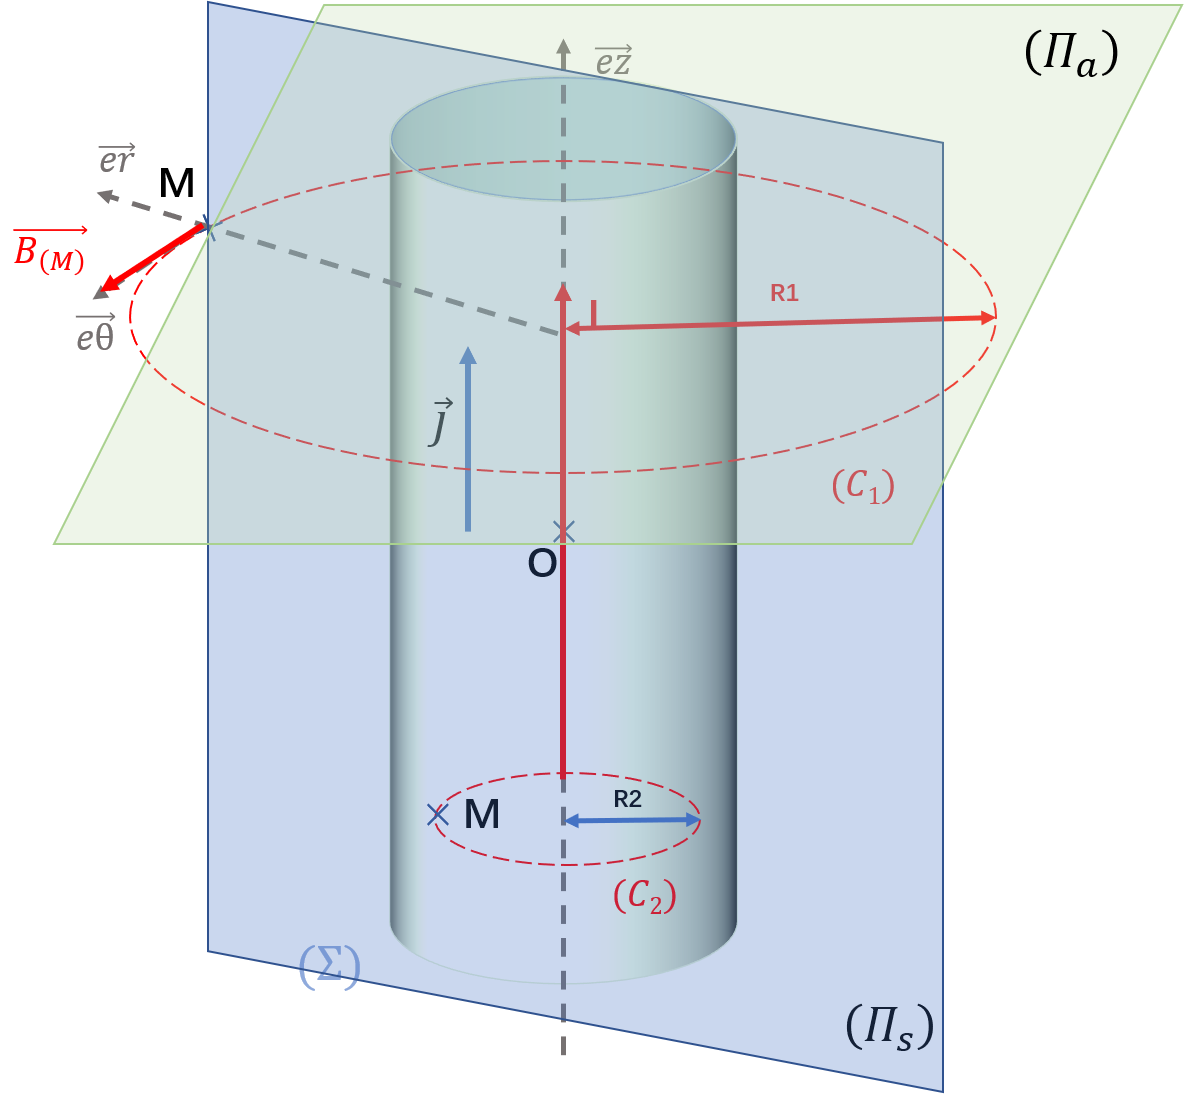
\includegraphics[scale=0.5]{elec22.png}
    \end{center}
    \caption{le système étudiée}
\end{figure}
\subsection{}
Le système $(\Sigma)$ étudiée: La distribution cylindrique de courant

% On a la charge élémentaire $\delta Q=\rho(P,t)\,d\tau_P$, avec $\rho(P,t)$ la densité volumique de charge.
% Pour une répartie uniformément et supposant que la charge est indépendant du temps, on a $\rho(P,t)=\rho$

% Dans le modèle d'une distribution de charge continue, on a 
% $$
% Q_{tot}=e=\iiint_{P \in (\Sigma)} \rho\,d\tau_P=\rho\iiint_{P \in (\Sigma)}d\tau_P=\frac{4}{3}\pi R^3\rho
% $$
% Donc la charge totale $\boxed{Q_{tot}=\frac{4}{3}\pi R^3\rho}$
On note $\vec{j}=j\vec{e}_z$ le vecteur densité volumique de courant est supposé uniforme et dirigé suivant Oz

On a l'intensité du courant électrique
$$
I=\iint_{M \in (S)}\vec{j}\cdot \overrightarrow{dS_M}=j\iint_{M \in (S)}dS=\pi R^2 j
$$
Donc on a $\vec{j}=\frac{I}{\pi R^2}\vec{e}_z$

On va employer les coordonnées cylindriques
\subsection{}
Pour un point $M=(r,\theta,z)$ quelconque, le système $(\Sigma)$ est symmétrique par rapport à $(\Pi_s)$ qui traverse $M$ et $\vec{e}_z$, donc $\overrightarrow{B(M)}$ est perpendiculaire à $(\Pi_s)$

$(\Sigma)$ est aussi antisymmétrique par rapport à $(\Pi_a)$ qui traverse $M$ et perpendiculaire à $\vec{e_z}$, donc $\overrightarrow{B(M)}$ appartient à $(\Pi_a)$. 

Ainsi, on a $\overrightarrow{B(M)}$ est selon la direction de $\vec{e}_\theta$, donc il s'écrit $\overrightarrow{B(M)}=B(r,\theta,z)\vec{e}_\theta$

Le système $(\Sigma)$ est invariante par rotation autour de l'axe $\vec{e}_z$, donc la norme du champ électrostatique $B(M)$ ne dépend que de l'angle : $\overrightarrow{B(M)}=B(r,z)\vec{e}_\theta$

Il est aussi invariante par translation selon $\vec{e}_z$, donc la norme $B(M)$ ne dépend de $z$, on a donc $\overrightarrow{B(M)}=B(r)\vec{e}_\theta$

\begin{itemize}
    \item Cas 1: Soit $M=(R_1,\theta,z)$ se trouve à l'extérieur de la cylindre, on pose $(\mathscr{C}_1)$ le contour fermée qui passe par $M$, avec le rayon $R_1\geq R$. 
    $(\mathscr{C}_1)$ est une surface iso-B comme tous les points sur $(\mathscr{C}_1)$ ont la même distance par rapport à $e_z$. 
    Donc on a la circulation qui traverse $(\mathscr{C}_1)$
    $$
    C_1=\oint_{M \in (\mathscr{C}_1)} \overrightarrow{B(M)}\cdot \overrightarrow{dl_M}=\oint_{M \in (\mathscr{C}_1)} B(R_1)\vec{e}_\theta \cdot dl\vec{e}_\theta=2\pi R_1B(R_1)
    $$
    et selon le théorème d'Ampère, on a aussi
    $$
    C_1=\mu_0 I_{int}=\mu_0 I
    $$
    On a donc 
    $$
    2\pi R_1 B(R_1)=\mu_0 I
    $$
    d'où
    $$
    \boxed{B(R_1)=\frac{\mu_0 I}{2\pi R_1}}
    $$
    \item Cas 2: Soit $M=(R_2,\theta,z)$ se trouve à l'intérieur de la cylindre, on pose $(\mathscr{C}_2)$ le contour fermée qui passe par $M$, avec le rayon $R_2 < R$. 
    $(S_2)$ est une surface iso-B comme tous les points sur $(\mathscr{C}_2)$ ont la même distance par rapport à $e_z$. 
    Donc on a la circulation qui traverse $(\mathscr{C}_2)$
    $$
    C_2=\oint_{M \in (\mathscr{C}_2)} \overrightarrow{B(M)}\cdot \overrightarrow{dl_M}=\oint_{M \in (\mathscr{C}_2)} B(R_2)\vec{e}_\theta\cdot dl\vec{e}_\theta=2\pi R_2B(R_2)
    $$
    et selon le théorème d'Ampère, on a aussi
    $$
    C_2=I_{int}\mu_0=\frac{\pi R_2^2}{\pi R^2}\mu_0 I
    $$
    On a donc 
    $$
    2\pi R_2B(R_2)=\frac{ R_2^2}{ R^2}\mu_0 I
    $$
    d'où
    $$
    \boxed{B(R_2)=\frac{R_2}{2\pi R^2}\mu_0 I}
    $$
\end{itemize}
On a donc pour $M=(r,\theta,z)$ quelconque
\begin{equation}  \nonumber
    \boxed{\overrightarrow{B(M)}=\left\{  
                 \begin{array}{rcl}  
                    \frac{\mu_0 I}{2\pi r}\vec{e}_\theta & & r \geq R\\
                    \frac{\mu_0 I r}{2\pi R^2}\vec{e}_\theta & & 0\leq r<R\\
                 \end{array}  
    \right.  }
\end{equation}
On notice que $\overrightarrow{B(M)}$ est continue en $r=R$



\end{document}